\documentclass[../thesis.tex]{subfiles}

\begin{document}


% Deep IRL in off-road environment

Most of the robotics problems can be solved under optimization framework. 
For the motion planning problem, the objective is to find a sequence of control actions that minimizes the accumulated costs toward the goal state. 
Reinforcement learning on the other hand formulates the problem as finding a policy that maximizes the expected accumulated rewards collected from the environment. 
Both problems require a definition of the cost/reward function of the interested robotics tasks.
However, unlike in the urban environment where cost function can be well defined in a rule-based structure, finding a cost function for off-road navigation can be nontrivial and often requires lot of handy tuning. \cite{silver2010learning}
Here, motivated by the recent successes \cite{wulfmeier2015maximum,wulfmeier2016watch} to using deep neural net to approximate the cost function, we implemented a similar algorithm for off-road application. 


\section{Proposed Methods}

\begin{figure}[t]
	\begin{center}
		\centerline{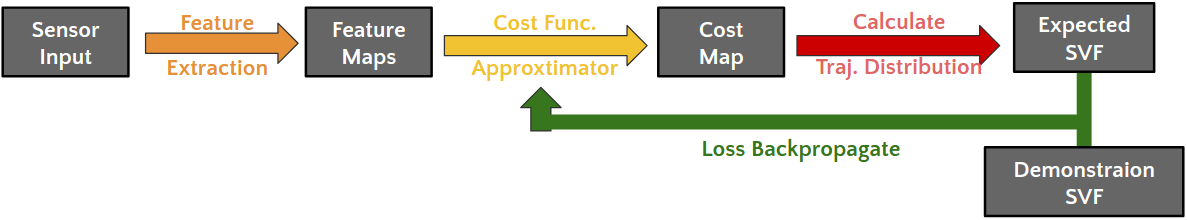
\includegraphics[width=\columnwidth]{./DIRL/fig/dirl_diagram.png}}
		\caption{Block diagram of deep inverse reinforcement learning.}
		\label{fig:dirl_diagram}
	\end{center}
\end{figure} 

The pipeline of deep inverse reinforcement learning (DIRL) is shown in Fig. \ref{fig:dirl_diagram}. 
The raw sensor inputs first process through the feature extraction module. 
The resulting feature maps stand as the inputs of the deep neural network that approximate the cost function.
Once the cost map is generated, we can formulate the corresponding Markov Decision Process (MDP) problem and solve for the expected state-visited frequencies (SVF).
Finally, we compare the expected SVF inferred under the current reward structure with the target SVF calculated from the demonstrations, and the gradient is applied using Eq. \ref{equ:dirl_grad}. 

\subsection{Learning from Failure for DIRL}

%%% Challenge %%% 
The fundamental challenge rises with DIRL is the spatially sparse gradient feedback. 
Since the gradient signals mainly and only come from the difference between demonstrations and expected trajectories, the loss feedbacks in training will inevitably focus more on the traversible regions.
% Since the gradient comes from the difference between two demonstration and maximum entropy distribution, the neural network will inherently focus more around the sample data. 
The problem can be alleviated by pre-training the network under standard image segmentation framework \cite{wulfmeier2016incorporating}, which provide a pixel-wise feedback for error terms. 
Here, we propose an alternative approach that re-formulated the some problem with \textit{negative} demonstrations.

Following the same convention in Section \ref{sec:dirl_intro}, we now denote the positive and negative demonstrations as $D_{pos}$ and $D_{neg}$, respectively. The log likelihood (Eq. \ref{equ:dirl_obj}) can be reformulated as:

\begin{align}
L(\theta) &= \log P(D_{pos}, D_{neg},\theta|r) \\
&= \log P(D_{pos}|r) + \log P(D_{neg}|r^{-1}) + \log P(\theta)
\end{align}

With the L2-regularization, the new gradient descent becomes:

\begin{align}
\frac{\partial L}{\partial \theta} &= \left( \mu_{D_{pos}} - \mathbb{E}_{r}[\mu] \right) \frac{\partial r}{\partial \theta} + \left( \mu_{D_{neg}} - \mathbb{E}_{r^{-1}}[\mu] \right) \frac{\partial r^{-1}}{\partial r} \frac{\partial r}{\partial \theta} + \frac{\lambda}{2} \| \theta \|^2 \\
&= \left( \mu_{D_{pos}} - \mathbb{E}_{r}[\mu] + \mathbb{E}_{r^{-1}}[\mu] - \mu_{D_{neg}} \right) \cdot \frac{\partial r}{\partial \theta} + \frac{\lambda}{2} \| \theta \|^2
\end{align}

where $r^{-1} = constant - r $ stands for the \textit{inverted} reward map. 
By jointly optimizing with the negative demonstrations, we can increase the gradient feedbacks for non-traversible regions where the positive demonstrations will never capture.

\subsection{Modeling Optimality Ambiguity}

As described in Section \ref{sec:dirl_intro}, the objective function of IRL is usually formulated either in a fashion of structured support vector machines (SSVM), or conditional random fields (CRFs). 
While Maximum Margin Planning (MMP) fall in the first category, Maximum Entropy IRL (ME-IRL) can represent the second category. 
However, both categories share a similar form on the gradient of its objective. 
Recall Eq. \ref{equ:mmp_obj} and Eq. \ref{equ:dirl_grad}, while gradient of MMP involves in solving the \textit{optimal} trajectory on the evolving reward map, the gradient of ME-IRL instead requires solving the \textit{expectation} of the trajectory distribution. 
The rest remains mostly the same.
\citet{pletscher2010entropy} proposed a generalized loss that models the observed expert behaviors with Gibbs distribution with an inverse temperature $\beta \in \mathbb R^{+}$. 

\begin{align}
P_{\beta}(\xi_i | r_\theta) &= \frac{1}{Z_\beta} \exp \left( \beta r_\theta(\xi_i) \right) \\
\text{,where \quad} Z_\beta &= \sum_{\xi \in \Xi} \exp \left( \beta r_\theta(\xi) \right) \text{is the normalization constant.}
\end{align}

As $\beta$ increases, the exponent term dominates, and the corresponding distribution become sharper. 
If $\beta \to \infty$, the distribution degenerates to solving the $\arg\max$, i.e. solving the optimal trajectory. 
On the other hand, if $\beta \to 1$, the distribution becomes the same form of the one used in ME-IRL.
In other words, the SSVM-like and CRF-like losses are framed under the same framework, and can be seen as two special cases located at the opposite side of the spectrum. 

This generalized loss introduces a new parameter $\beta$ that captures on which level of the \textit{optimality} is presented by the demonstration trajectories. By using this generalized loss in our computational graph, the parameter can be optimized jointly during training.

\section{Experiments Results}

\begin{figure}[t]
	\begin{center}
		\centerline{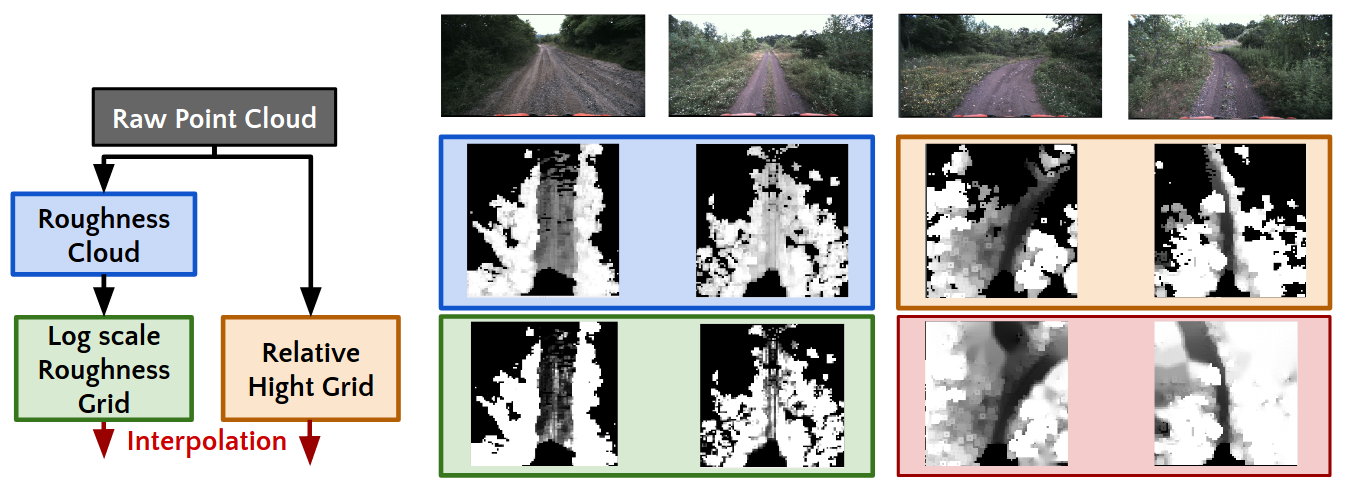
\includegraphics[width=\columnwidth]{./DIRL/fig/lidar_feature_map.png}}
		\caption{The extracted feature maps from LiDAR. The flow chart is shown on the left of the figure, while examples of the actual collected data on filed are shown on the right of the figure.}
		\label{fig:lidar_feature_map}
	\end{center}
\end{figure} 


\begin{figure}[t]
	\begin{center}
		\centerline{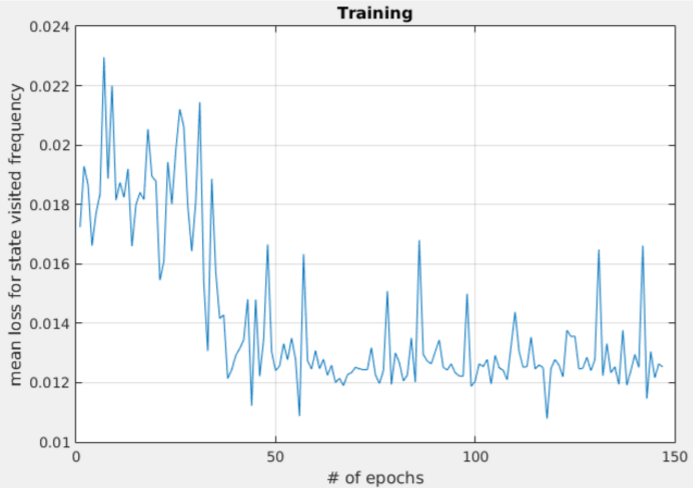
\includegraphics[width=0.5\columnwidth]{./DIRL/fig/dirl_training_curve.png}}
		\caption{Training curve of DIRL in Gascola dataset.}
		\label{fig:dirl_learning_curve}
	\end{center}
\end{figure} 

\begin{figure}[t]
	\begin{center}
		\centerline{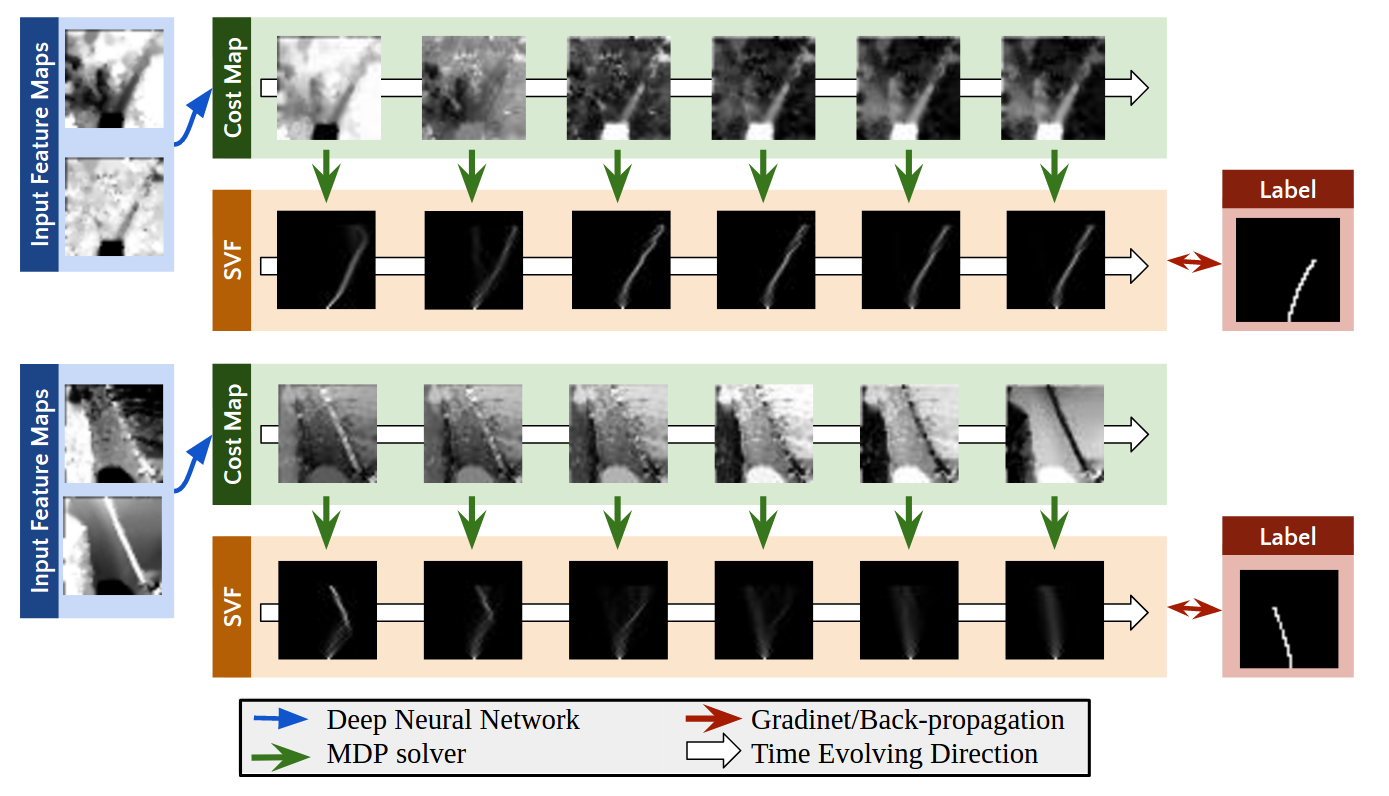
\includegraphics[width=\columnwidth]{./DIRL/fig/inter_cost_map.png}}
		\caption{Samples of intermediate cost maps during training.}
		\label{fig:inter_cost_map}
	\end{center}
\end{figure} 

\begin{figure}[t]
	\begin{center}
		\centerline{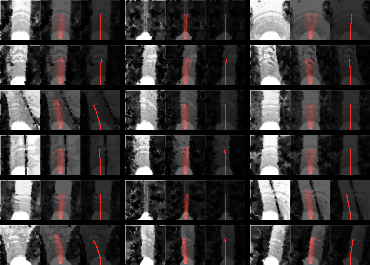
\includegraphics[width=0.8\columnwidth]{./DIRL/fig/gradtestImg040.png}}
		\caption{Final cost map on testing set. The left, middle, and right image represent the output cost map, the same cost map overlapped with expected SVF, and with demonstrations, respectively.}
		\label{fig:final_cost_map}
	\end{center}
\end{figure} 

Following the similar setup in Chapter \ref{chap:rrtplanner}, we use Yamaha Viking VI side-by-side ATV as our main testing platform, with LiDAR as our primary input sensor. 
For off-road navigation where scenes can change dramatically, LiDAR usually provides a more reliable measurement for the safety concern.
In addition, informative features such as terrain roughness can be inferred straight-forwardly.
We collect the dataset with total 150 human demonstrations covering an off-road testing field at Gascola, PA. Each sample covers the $20m \times 20m$ region in the front of the ATV. Since the Gascola dataset is relatively small, we use a shallow multilayer perception as the cost function. 

The first feature map captures information about terrain roughness.
As shown in Fig. \ref{fig:lidar_feature_map}, the basic approach to infer the terrain roughness from the raw point cloud is to first divide it into patches. 
For each patch, a normal plane is fitted using standard least square regression. 
Once the plane parameters is calculated, the \textit{roughness index} can be inferred by averaging plane variance within each patch. 
However, this naive roughness index is sensitive to hyper-parameter such as patch size and rescaling factors. 
In the off-road environment where terrain types can vary a lot, this approach can fail to extract reasonable feature when trail becomes narrow, as shown in the second column of Fig. \ref{fig:lidar_feature_map}. 
To alleviate this issue, we transfer the original roughness index with the log-scale value. 
The log scale helps amplify the slight difference among traversible terrains, in which we are in general more interested.
On the other hand, the non-traversible terrains such as bush or trees are flattened under the log scale. 
Another informative feature map is the relative hight with respect to the vehicle standing level. 


The intuition behind the two feature maps is that the vehicle should prefer driving over the terrains that are smoother or at the similar horizontal level of its current local frame.
Note that both of the feature maps are projected on a top-down view, leaving some parts of the feature maps unoccupied. 
However, the invisible grids may confuse the network and make the framework fragile to the senses. 
Though the problem can be alleviated by simply providing an additional feature map that specifies the visibility, it usually requires much more data and the use of convolution layer. \cite{wulfmeier2015maximum,wulfmeier2016watch}
Since our dataset is relatively small, we alleviate this issue with an alternative approach. 
Instead, we apply a standard image in-painting technique \cite{telea2004image} that effectively helps infer the invisible region given the geometric shape of the visible trails. 
The feature maps before and after the interpolation are shown in the orange and red area in Fig. \ref{fig:lidar_feature_map}, respectively.

The training curve is summarized in Fig. \ref{fig:dirl_learning_curve}, and two testing examples of the intermediate cost maps during training are visualized in Fig. \ref{fig:inter_cost_map}. Fially, the resulting cost map on testing data set is shown in Fig. \ref{fig:final_cost_map}.

\end{document}